\documentclass[10pt]{IEEEtran}
\usepackage[spanish]{babel}
\usepackage[utf8]{inputenc}
\usepackage{graphicx}
\usepackage{subfigure} 
\usepackage{amsmath}
\usepackage{float}



\title {Operación XOR de manera cruzada en mapas Renyi donde $ 1 \leq j \leq 10$,  valores diferentes para el parámetro $\beta$, aplicación de pruebas NIST.}

\author{\IEEEauthorblockN{Marcos Daniel Calderón Calderón}\\
\IEEEauthorblockA{Maestría en Ciencias de la Computación\\
Centro de Investigación en Matemáticas (CIMAT)\\
Guanajuato , Gto.\\
marcos.calderon@cimat.mx}}


\begin{document}
\maketitle
\begin{abstract}
Se explica de manera detallada el comportamiento de mapas Renyi donde varía el parámetro $j$.
\end{abstract}
\section{Introducción.}

Para este ejercicio, se trabajó con el mapa caótico Renyi fundamental:


\begin{equation}
f(k)=  \left(  bk +  \lfloor \frac{k}{2^{j}} \rfloor   \right) \mod{ 2^{n}}
\end{equation}.

Esto significa que es importante buscar valor adecuado para $b$. Se tienen algunas restricciones para el valor de $b$ que son mencionadas a continuación:

\begin{enumerate}
\item Se debe cumplir que $1 \leq b < 2^{n}$.
\end{enumerate}

Ahora, para facilitar la explicación, supongamos que estamos trabajando con datos de 8 bits. Esto significa que cada número se puede dividir en dos partes de 4 bits, la parte izquierda es la más significativa, la parte derecha es la menos significativa. Supongamos que vamos a trabajar con los siguientes datos:

\begin{equation}
x_{1}=103 \quad    (0110 0111)
\quad \quad 
x_{2}=89 \quad     (0101 1001)
\end{equation}


También, necesitamos un valor auxiliar:
\begin{equation}
a=15  \quad  \quad   (0000 1111)
\end{equation}

El esquema que se manejará es el siguiente:
\begin{figure}[H]
\centering
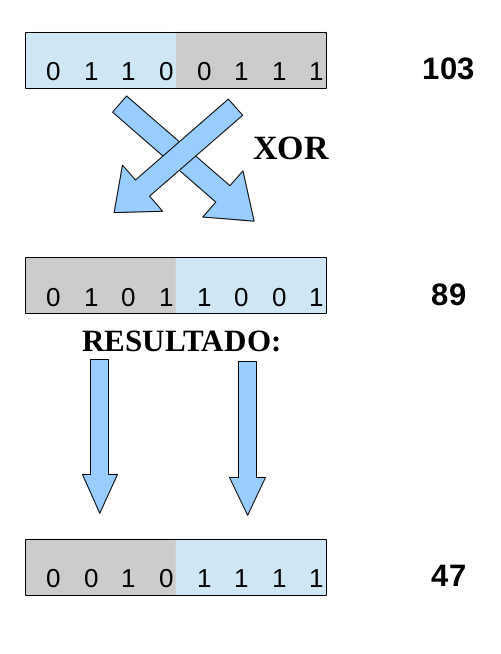
\includegraphics[width=7cm]{es.jpg}
\caption{Esquema de intercambio.}
\label{vovo}
\end{figure}

Un código simplificado (para ocho bits) que hace la operación anterior es el siguiente:
\begin{verbatim}

   char a = 15;
   char temp;
   char temp1;
   char temp2;
   char Xn1;
   char Xn2;
   char Xn3;
   Xn1=103;
   Xn2= 89;
            temp1 = Xn2 & a;
            temp2 = Xn1 >> 4;
            temp = temp1^temp2;
            temp1 = Xn2 >> 4;
            temp2 = Xn1 & a;
            Xn3=(temp1^temp2)<<4;
            Xn3|=temp;
\end{verbatim}


Ahora, para los ejemplos que se muestran aquí se utilizan 32 bits, esto significa que se van a dividir los datos generados por los mapas caóticos en dos partes: cada una de 16 bits. También, en este caso, necesitamos un nuevo valor para a: $(a = 2^{16}-1= 65,535)$



Todos los números impares $i$ tales que $i < 2^{32}$ son coprimos con $ 2^{32}$.
 
\section{Resultados.}

\subsection{Ejemplo 1.}
Se eligieron los siguientes parámetros fijos para el valor de $b$:

\begin{itemize}
\item Mapa 1: $b =  5$.
\item Mapa 2: $b =  5$.
\end{itemize}

También, se han elegido los siguientes valores iniciales, recordemos que al ser mapas caóticos, no importa que los valores iniciales se encuentren cerca, con el paso de las iteraciones, se obtentrán resultados muy distintos.

\begin{itemize}
\item Mapa 1: $x_{0} = 7$.
\item Mapa 2: $x_{0} = 9$.
\end{itemize}




\begin{table}[H]
\caption{Resultados de las pruebas de aleatoriedad NIST a los datos ej1.dat .}
\label{caso1}
\begin{center}
\begin{small}
\begin{tabular}{|l|c|r|}
\hline

Prueba Aplicada &  P-Valor & Exito? \\
\hline

Aproximate Entropy    &    0.521549  & $\surd$ \\

Block Frecuency  & 0.418270  &  $\surd$  \\

Cumulative Sums    &   F:0.826938, R:0.625796  & $\surd$ \\

FFT    &   0.408863 &  $\surd$     \\

Frecuency     &  0.477704  &  $\surd$   \\

Linear Complexity      & 0.352064 & $\surd$ \\

Longest Run      &   0.453277 &    $\surd$      \\

Non Overlapping Template      & 147 de 148    &     $\surd$          \\

Overlapping Template      &  0.103749   &      $\surd$      \\

Random Excursions      & 8 de 8  &    $\surd$      \\

Random Excursions Variant & 18 de 18 &     $\surd$    \\

Rank &  0.404006 &      $\surd$      \\

Runs &    0.910677 &     $\surd$        \\

Serial &     2 de 2    &     $\surd$        \\

Universal &     0.445230  &   $\surd$            \\

\hline

\end{tabular}
\end{small}
\end{center}
\end{table}





\subsection{Ejemplo 2.}
En este segundo ejemplo, se utilizó un valor para $b$ de tipo par, además dicho valor tiene una representación de la forma $2^{n}$.:

\begin{itemize}
\item Mapa 1: $b =  128$.
\item Mapa 2: $b =  128$.
\end{itemize}

Los valores iniciales son los mismos que los utilizados en el ejemplo anterior.
\begin{itemize}
\item Mapa 1: $x_{0} = 7$.
\item Mapa 2: $x_{0} = 9$.
\end{itemize}




\begin{table}[H]
\caption{Resultados de las pruebas de aleatoriedad NIST a los datos ej2.dat .}
\label{caso1}
\begin{center}
\begin{small}
\begin{tabular}{|l|c|r|}
\hline

Prueba Aplicada &  P-Valor & Exito? \\
\hline

Aproximate Entropy    &    0.499866  & $\surd$ \\

Block Frecuency  & 0.864971 &  $\surd$  \\

Cumulative Sums    &   F:0.552499, R:0.393020  & $\surd$ \\

FFT    &   0.967975 &  $\surd$     \\

Frecuency     & 0.457784  &  $\surd$   \\

Linear Complexity      & 0.330454 & $\surd$ \\

Longest Run      &  0.577948 &    $\surd$      \\

Non Overlapping Template      & 147 de 148    &     $\surd$          \\

Overlapping Template      &  0.590943   &      $\surd$      \\

Random Excursions      & 8 de 8  &    $\surd$      \\

Random Excursions Variant & 18 de 18 &     $\surd$    \\

Rank &  0.118981 &      $\surd$      \\

Runs &    0.560840 &     $\surd$        \\

Serial &     2 de 2    &     $\surd$        \\

Universal &     0.587190 &   $\surd$            \\

\hline

\end{tabular}
\end{small}
\end{center}
\end{table}



\subsection{Ejemplo 3.}
Se eligieron los siguientes parámetros fijos para el valor de $b$:

\begin{itemize}
\item Mapa 1: $b =  5$.
\item Mapa 2: $b =  5$.
\end{itemize}

También, se han elegido los siguientes valores iniciales, a diferencia del ejemplo 1, en este caso, los valores iniciales difieren mucho entre si:

\begin{itemize}
\item Mapa 1: $x_{0} = 7$.
\item Mapa 2: $x_{0} =123,879,573$.
\end{itemize}




\begin{table}[H]
\caption{Resultados de las pruebas de aleatoriedad NIST a los datos ej3.dat .}
\label{caso1}
\begin{center}
\begin{small}
\begin{tabular}{|l|c|r|}
\hline

Prueba Aplicada &  P-Valor & Exito? \\
\hline

Aproximate Entropy    &     0.343785  & $\surd$ \\

Block Frecuency  & 0.996993  &  $\surd$  \\

Cumulative Sums    &   F:0.072120, R:0.024275 & $\surd$ \\

FFT    &   0.189046 &  $\surd$     \\

Frecuency     &  0.045097  &  $\surd$   \\

Linear Complexity      & 0.969194 & $\surd$ \\

Longest Run      &   0.238385 &    $\surd$      \\

Non Overlapping Template      & 147 de 148    &     $\surd$          \\

Overlapping Template      &  0.892500   &      $\surd$      \\

Random Excursions      & 8 de 8  &    $\surd$      \\

Random Excursions Variant & 18 de 18 &     $\surd$    \\

Rank & 0.128193  &      $\surd$      \\

Runs &    0.389105 &     $\surd$        \\

Serial &     2 de 2    &     $\surd$        \\

Universal &     0.913238  &   $\surd$            \\

\hline

\end{tabular}
\end{small}
\end{center}
\end{table}




\subsection{Ejemplo 4.}
Para el ejemplo 4, se tomó como referencia los parámetros iniciales del ejemplo 1, pero ahora, en el primer mapa, se asignará  $j=3$, esto significa que los mapas no coincidirán en este parámetro.



\begin{itemize}
\item Mapa 1: $j =  3$.
\item Mapa 2: $j =  5$.
\end{itemize}

Para este ejemplo, el valor del parámetro es el mismo para ambos mapas:

\begin{itemize}
\item Mapa 1: $b =  5$.
\item Mapa 2: $b =  5$.
\end{itemize}

También, se han elegido los siguientes valores iniciales, recordemos que al ser mapas caóticos, no importa que los valores iniciales se encuentren cerca, con el paso de las iteraciones, se obtentrán resultados muy distintos.

\begin{itemize}
\item Mapa 1: $x_{0} = 7$.
\item Mapa 2: $x_{0} = 9$.
\end{itemize}




\begin{table}[H]
\caption{Resultados de las pruebas de aleatoriedad NIST a los datos ej4.dat .}
\label{caso1}
\begin{center}
\begin{small}
\begin{tabular}{|l|c|r|}
\hline

Prueba Aplicada &  P-Valor & Exito? \\
\hline

Aproximate Entropy    &    0.325726  & $\surd$ \\

Block Frecuency  & 0.713352  &  $\surd$  \\

Cumulative Sums    &   F:0.586388, R:0.421338 & $\surd$ \\

FFT    &   0.858882 &  $\surd$     \\

Frecuency     &  0.414357  &  $\surd$   \\

Linear Complexity      &  0.460441  & $\surd$ \\

Longest Run      &   0.048773  &    $\surd$      \\

Non Overlapping Template      & 146 de 148    &     $\surd$          \\

Overlapping Template      &  0.079603   &      $\surd$      \\

Random Excursions      & 8 de 8  &    $\surd$      \\

Random Excursions Variant & 14 de 18 &     $\surd$    \\

Rank & 0.979570 &      $\surd$      \\

Runs &    0.447753  &     $\surd$        \\

Serial &     2 de 2    &     $\surd$        \\

Universal &     0.927187  &   $\surd$            \\

\hline

\end{tabular}
\end{small}
\end{center}
\end{table}



\subsection{Ejemplo 5.}
Este ejemplo es similar al caso 1, pero aquí se ha modificado el valor de $j$: los dos mapas utilizarán $j=1$. En teoría, se supone que con este cambio, es posible generar más valores. Se eligieron los siguientes parámetros fijos para el valor de $b$:

\begin{itemize}
\item Mapa 1: $b =  5$.
\item Mapa 2: $b =  5$.
\end{itemize}

También, se han elegido los siguientes valores iniciales, recordemos que al ser mapas caóticos, no importa que los valores iniciales se encuentren cerca, con el paso de las iteraciones, se obtentrán resultados muy distintos.

\begin{itemize}
\item Mapa 1: $x_{0} = 7$.
\item Mapa 2: $x_{0} = 9$.
\end{itemize}




\begin{table}[H]
\caption{Resultados de las pruebas de aleatoriedad NIST a los datos ej5.dat .}
\label{caso1}
\begin{center}
\begin{small}
\begin{tabular}{|l|c|r|}
\hline

Prueba Aplicada &  P-Valor & Exito? \\
\hline

Aproximate Entropy    &    0.674153  & $\surd$ \\

Block Frecuency  &  0.282417  &  $\surd$  \\

Cumulative Sums    &   F:0.059542, R:0.036427 & $\surd$ \\

FFT    &   0.189046   &  $\surd$     \\

Frecuency     &  0.059093  &  $\surd$   \\

Linear Complexity      & 0.507308 & $\surd$ \\

Longest Run      &   0.216161  &    $\surd$      \\

Non Overlapping Template      & 146 de 148    &     $\surd$          \\

Overlapping Template      &   0.280685   &      $\surd$      \\

Random Excursions      & 8 de 8  &    $\surd$      \\

Random Excursions Variant & 18 de 18 &     $\surd$    \\

Rank & 0.690115  &      $\surd$      \\

Runs &   0.945406  &     $\surd$        \\

Serial &     2 de 2    &     $\surd$        \\

Universal &     0.819727 &   $\surd$            \\

\hline

\end{tabular}
\end{small}
\end{center}
\end{table}


\subsection{Ejemplo 6.}
Este ejemplo es similar al caso 1 y al caso 5, pero aquí se ha modificado el valor de $j$: los dos mapas utilizarán $j=2$. 

\begin{itemize}
\item Mapa 1: $b =  5$.
\item Mapa 2: $b =  5$.
\end{itemize}

También, se han elegido los siguientes valores iniciales:

\begin{itemize}
\item Mapa 1: $x_{0} = 7$.
\item Mapa 2: $x_{0} = 9$.
\end{itemize}




\begin{table}[H]
\caption{Resultados de las pruebas de aleatoriedad NIST a los datos ej6.dat .}
\label{caso1}
\begin{center}
\begin{small}
\begin{tabular}{|l|c|r|}
\hline

Prueba Aplicada &  P-Valor & Exito? \\
\hline

Aproximate Entropy    &    0.128491  & $\surd$ \\

Block Frecuency  & 0.264198  &  $\surd$  \\

Cumulative Sums    &   F:0.820872, R:0.660928 & $\surd$ \\

FFT    &   0.679644  &  $\surd$     \\

Frecuency     &  0.812269  &  $\surd$   \\

Linear Complexity      & 0.578214 & $\surd$ \\

Longest Run      &   0.699453 &    $\surd$      \\

Non Overlapping Template      & 145 de 148    &     $\surd$          \\

Overlapping Template      &   0.768770  &      $\surd$      \\

Random Excursions      & 8 de 8  &    $\surd$      \\

Random Excursions Variant & 18 de 18 &     $\surd$    \\

Rank & 0.548353 &      $\surd$      \\

Runs &    0.764204  &     $\surd$        \\

Serial &     2 de 2    &     $\surd$        \\

Universal &    0.468438  &   $\surd$            \\

\hline

\end{tabular}
\end{small}
\end{center}
\end{table}




\subsection{Ejemplo 7.}
Este ejemplo es similar al caso 1 y al caso 5, pero aquí se ha modificado el valor de $j$: los dos mapas utilizarán $j=3$. 

\begin{itemize}
\item Mapa 1: $b =  5$.
\item Mapa 2: $b =  5$.
\end{itemize}

También, se han elegido los siguientes valores iniciales:

\begin{itemize}
\item Mapa 1: $x_{0} = 7$.
\item Mapa 2: $x_{0} = 9$.
\end{itemize}




\begin{table}[H]
\caption{Resultados de las pruebas de aleatoriedad NIST a los datos ej7.dat .}
\label{caso1}
\begin{center}
\begin{small}
\begin{tabular}{|l|c|r|}
\hline

Prueba Aplicada &  P-Valor & Exito? \\
\hline

Aproximate Entropy    &   0.405724  & $\surd$ \\

Block Frecuency  &  0.432030  &  $\surd$  \\

Cumulative Sums    &   F:0.673151, R:0.452943 & $\surd$ \\

FFT    &   0.895052 &  $\surd$     \\

Frecuency     &  0.546010 &  $\surd$   \\

Linear Complexity      & 0.655230& $\surd$ \\

Longest Run      &  0.156917 &    $\surd$      \\

Non Overlapping Template      & 147 de 148    &     $\surd$          \\

Overlapping Template      &  0.253751  &      $\surd$      \\

Random Excursions      & 8 de 8  &    $\surd$      \\

Random Excursions Variant & 16 de 18 &     $\surd$    \\

Rank & 0.366550  &      $\surd$      \\

Runs &   0.215522  &     $\surd$        \\

Serial &     2 de 2    &     $\surd$        \\

Universal &   0.683250  &   $\surd$            \\

\hline

\end{tabular}
\end{small}
\end{center}
\end{table}






\subsection{Ejemplo 8.}
Similar al caso y, pero aquí se ha modificado el valor de $j$: los dos mapas utilizarán $j=4$. 

\begin{itemize}
\item Mapa 1: $b =  5$.
\item Mapa 2: $b =  5$.
\end{itemize}

También, se han elegido los siguientes valores iniciales:

\begin{itemize}
\item Mapa 1: $x_{0} = 7$.
\item Mapa 2: $x_{0} = 9$.
\end{itemize}




\begin{table}[H]
\caption{Resultados de las pruebas de aleatoriedad NIST a los datos ej8.dat .}
\label{caso1}
\begin{center}
\begin{small}
\begin{tabular}{|l|c|r|}
\hline

Prueba Aplicada &  P-Valor & Exito? \\
\hline

Aproximate Entropy    &   0.237421  & $\surd$ \\

Block Frecuency  &   0.008199 &  $X$  \\

Cumulative Sums    &   F:0.387010, R:0.354730 & $\surd$ \\

FFT    &   0.688069 &  $\surd$     \\

Frecuency     &  0.349144 &  $\surd$   \\

Linear Complexity      & 0.290362 & $\surd$ \\

Longest Run      &  0.440753 &    $\surd$      \\

Non Overlapping Template      & 147 de 148    &     $\surd$          \\

Overlapping Template      &  0.072547  &      $\surd$      \\

Random Excursions      & 8 de 8  &    $\surd$      \\

Random Excursions Variant & 18 de 18 &     $\surd$    \\

Rank & 0.667748  &      $\surd$      \\

Runs &   0.190805  &     $\surd$        \\

Serial &     2 de 2    &     $\surd$        \\

Universal &   0.188711 &   $\surd$            \\

\hline

\end{tabular}
\end{small}
\end{center}
\end{table}




\subsection{Ejemplo 9.}
Similar al caso 1, pero aquí se ha modificado el valor de $j$: los dos mapas utilizarán $j=6$. 

\begin{itemize}
\item Mapa 1: $b =  5$.
\item Mapa 2: $b =  5$.
\end{itemize}

También, se han elegido los siguientes valores iniciales:

\begin{itemize}
\item Mapa 1: $x_{0} = 7$.
\item Mapa 2: $x_{0} = 9$.
\end{itemize}




\begin{table}[H]
\caption{Resultados de las pruebas de aleatoriedad NIST a los datos ej9.dat .}
\label{caso9}
\begin{center}
\begin{small}
\begin{tabular}{|l|c|r|}
\hline

Prueba Aplicada &  P-Valor & Exito? \\
\hline

Aproximate Entropy    &   0.296938  & $\surd$ \\

Block Frecuency  &  0.518738 &   $\surd$   \\

Cumulative Sums    &   F:0.085992, R:0.309723 & $\surd$ \\

FFT    &   0.228422 &  $\surd$     \\

Frecuency     &  0.154881 &  $\surd$   \\

Linear Complexity      & 0.359101 & $\surd$ \\

Longest Run      &  0.568405 &    $\surd$      \\

Non Overlapping Template      & 146 de 148    &     $\surd$          \\

Overlapping Template      &  0.018236  &      $\surd$      \\

Random Excursions      & NA  &    $X$      \\

Random Excursions Variant & NA &     $X$    \\

Rank & 0.517635  &      $\surd$      \\

Runs &   0.596122  &     $\surd$        \\

Serial &     2 de 2    &     $\surd$        \\

Universal &   0.796828 &   $\surd$            \\

\hline

\end{tabular}
\end{small}
\end{center}
\end{table}


/////////////////

\subsection{Ejemplo 10.}
Valor de $j$: los dos mapas utilizarán $j=7$. 

\begin{itemize}
\item Mapa 1: $b =  5$.
\item Mapa 2: $b =  5$.
\end{itemize}

También, se han elegido los siguientes valores iniciales:

\begin{itemize}
\item Mapa 1: $x_{0} = 7$.
\item Mapa 2: $x_{0} = 9$.
\end{itemize}




\begin{table}[H]
\caption{Resultados de las pruebas de aleatoriedad NIST a los datos ej10.dat .}
\label{caso10}
\begin{center}
\begin{small}
\begin{tabular}{|l|c|r|}
\hline

Prueba Aplicada &  P-Valor & Exito? \\
\hline

Aproximate Entropy    &  0.608377  & $\surd$ \\

Block Frecuency  & 0.898356 &   $\surd$   \\

Cumulative Sums    &   F:0.529105, R:0.872757 & $\surd$ \\

FFT    &    0.335274   &  $\surd$     \\

Frecuency     &  0.513273  &  $\surd$   \\

Linear Complexity      & 0.035298 & $\surd$ \\

Longest Run      & 0.560911 &    $\surd$      \\

Non Overlapping Template      & 146 de 148    &     $\surd$          \\

Overlapping Template      &  0.565435  &      $\surd$      \\

Random Excursions      & NA  &    $X$      \\

Random Excursions Variant & NA &     $X$    \\

Rank &  0.365659  &      $\surd$      \\

Runs &   0.157147  &     $\surd$        \\

Serial &     2 de 2    &     $\surd$        \\

Universal &   0.988075 &   $\surd$            \\

\hline

\end{tabular}
\end{small}
\end{center}
\end{table}




\subsection{Ejemplo 11.}
Valor de $j$: los dos mapas utilizarán $j=8$. 

\begin{itemize}
\item Mapa 1: $b =  5$.
\item Mapa 2: $b =  5$.
\end{itemize}

También, se han elegido los siguientes valores iniciales:

\begin{itemize}
\item Mapa 1: $x_{0} = 7$.
\item Mapa 2: $x_{0} = 9$.
\end{itemize}




\begin{table}[H]
\caption{Resultados de las pruebas de aleatoriedad NIST a los datos ej11.dat .}
\label{caso11}
\begin{center}
\begin{small}
\begin{tabular}{|l|c|r|}
\hline

Prueba Aplicada &  P-Valor & Exito? \\
\hline

Aproximate Entropy    &   0.156682  & $\surd$ \\

Block Frecuency  &  0.145581 &   $\surd$   \\

Cumulative Sums    &   F:0.082204, R:0.097820 & $\surd$ \\

FFT    &   0.823006 &  $\surd$     \\

Frecuency     &  0.062533  &  $\surd$   \\

Linear Complexity      & 0.457037 & $\surd$ \\

Longest Run      &  0.789188  &    $\surd$      \\

Non Overlapping Template      & 144 de 148    &     $\surd$          \\

Overlapping Template      &  0.140399  &      $\surd$      \\

Random Excursions      & NA  &    $X$      \\

Random Excursions Variant & NA &     $X$    \\

Rank & 0.477033  &      $\surd$      \\

Runs &    0.101856  &     $\surd$        \\

Serial &     2 de 2    &     $\surd$        \\

Universal &   0.833920  &   $\surd$            \\

\hline

\end{tabular}
\end{small}
\end{center}
\end{table}




\subsection{Ejemplo 12.}
El valor de $j$: los dos mapas utilizarán $j=9$. 

\begin{itemize}
\item Mapa 1: $b =  5$.
\item Mapa 2: $b =  5$.
\end{itemize}

También, se han elegido los siguientes valores iniciales:

\begin{itemize}
\item Mapa 1: $x_{0} = 7$.
\item Mapa 2: $x_{0} = 9$.
\end{itemize}




\begin{table}[H]
\caption{Resultados de las pruebas de aleatoriedad NIST a los datos ej12.dat .}
\label{caso12}
\begin{center}
\begin{small}
\begin{tabular}{|l|c|r|}
\hline

Prueba Aplicada &  P-Valor & Exito? \\
\hline

Aproximate Entropy    &   0.225604  & $\surd$ \\

Block Frecuency  & 0.159517  &   $\surd$  \\

Cumulative Sums    &   F:0.360374, R:0.323347 & $\surd$ \\

FFT    &    0.692295  &  $\surd$     \\

Frecuency     & 0.353019 &  $\surd$   \\

Linear Complexity      & 0.036720 & $\surd$ \\

Longest Run      &   0.820065 &    $\surd$      \\

Non Overlapping Template      & 146 de 148    &     $\surd$          \\

Overlapping Template      & 0.046354  &      $\surd$      \\

Random Excursions      & 8 de 8  &    $\surd$      \\
Random Excursions Variant & 18 de 18 &     $\surd$    \\

Rank & 0.558845  &      $\surd$      \\

Runs &   0.440878 &     $\surd$        \\

Serial &     2 de 2    &     $\surd$        \\

Universal &  0.780192 &   $\surd$            \\

\hline

\end{tabular}
\end{small}
\end{center}
\end{table}




\subsection{Ejemplo 13.}
Valor de $j$: los dos mapas utilizarán $j=10$. 

\begin{itemize}
\item Mapa 1: $b =  5$.
\item Mapa 2: $b =  5$.
\end{itemize}

También, se han elegido los siguientes valores iniciales:

\begin{itemize}
\item Mapa 1: $x_{0} = 7$.
\item Mapa 2: $x_{0} = 9$.
\end{itemize}




\begin{table}[H]
\caption{Resultados de las pruebas de aleatoriedad NIST a los datos ej13.dat .}
\label{caso9}
\begin{center}
\begin{small}
\begin{tabular}{|l|c|r|}
\hline

Prueba Aplicada &  P-Valor & Exito? \\
\hline

Aproximate Entropy    &   0.455556 & $\surd$ \\

Block Frecuency  & 0.921870 &  $\surd$  \\

Cumulative Sums    &   F:0.687762, R:0.539668 & $\surd$ \\

FFT    &   0.613759 &  $\surd$     \\

Frecuency     &  0.810330 &  $\surd$   \\

Linear Complexity      & 0.253101 & $\surd$ \\

Longest Run      &  0.062643 &    $\surd$      \\

Non Overlapping Template      & 142 de 148    &     $\surd$          \\

Overlapping Template      &  0.468493  &      $\surd$      \\

Random Excursions      & 8 de 8  &   $\surd$      \\

Random Excursions Variant & 18 de 18 &    $\surd$     \\

Rank & 0.665825  &      $\surd$      \\

Runs &   0.737598  &     $\surd$        \\

Serial &     2 de 2    &     $\surd$        \\

Universal &   0.309633 &   $\surd$            \\

\hline

\end{tabular}
\end{small}
\end{center}
\end{table}







\section{Conclusiones.}


Cuando se asigna el parámetro $b$ como se ha hecho en este ejemplo, se puede asignar el mismo valor a los dos mapas caóticos que participarn en la operación $XOR$, lo único que se necesita para obtener buenos resultados es asignar valores distintos a $x_{0}$, estos valores pueden estar muy cerca entre sí, el comportamiento caótico asegura que aún así, la secuencia obtenida será aleatoria.


Se obtuvieron mejores resultados  (ligeramente) mejores en el ejemplo 1 en comparación con el ejemplo 2. Quizá esto se debe a que en el ejemplo 1 se utilizó un primo relativo con respecto a $b$.

En el ejemplo 3, los valores iniciales fueron muy distintos entre sí, a pesar de que se aprobaron los exámenes de aleatoriedad, los resultados no fueron tan buenos como en el ejemplo 1.

En el ejemplo 4, a pesar de que los rsultados no fueron malos, no fueron tan bueno es comparación con ejemplos anteriores, algunas pruebas obtivieron valores relativamente bajos en comparación con los experimentos de pruebas anteriores.

En el ejemplo 5, donde $j=1$, se obtuvieron buenos resultados, aunque la prueba de Frecuencia obtuvo un valor bajo, esto indica que el número de ceros y unos no está bien nivelado. También se obtuvieron algunas pruebas  Non Overlapping Template, otra prueba que obtuvo resultados apenas aceptables fué Cumulative Sums.  


En el ejemplo 6, se obtuvieron buenos resultados, pero, hubo dos pruebas con reultados no tan buenos: Serial y Non Overlapping Template.

En el ejemplo 7, Random Excursions Variant fué la prueba con menor desempeño.

En el ejemplo 8, la Prueba Frecuency Block ha fallado.

En el ejemplo 9, hay unas pruebas que no se pueden aplicar, pero esto se debe a las especificaciones del programa.

Ejemplo 12 y 13, buenos resultados.

En general, se obtienen buenos resultados para $5 \leq j \leq 10$. Además, se obtienen mejores resultados cuando no se utiliza la fórmula para el parámetro $b$.
\end{document}


